\capitulo{6}{Trabajos relacionados}

\section{Juegos similares en género y mecánicas}
Este videojuego se inspira de otros dos videojuegos diferentes: Super Meat Boy \footnote{Enlace a la página de Wikipedia de Super Meat Boy: \url{https://es.wikipedia.org/wiki/Super_Meat_Boy}} y Celeste 
\footnote{Enlace a la página de Wikipedia de Celeste: \url{https://es.wikipedia.org/wiki/Celeste_(videojuego)}}. Esta temática es a nivel de género más que de mecánicas. Ambos juegos son plataformas 2D comprometidos con sus mecánicas y precisos en su jugabilidad (esto es lo que se busca con el proyecto que se va a desarrollar). Es cierto que Celeste está más comprometida con la historia que Super Meat Boy, mientras este se centra casi exclusivamente en las mecánicas.

Celeste representa la variedad mecánica que se desea alcanzar, ofreciendo mecánicas distintas como acelerones y portales (igual que el videojuego que se va a desarrollar) e incluso mecánicas que modifican el estado natural del juego (como permitir dar más de un acelerón en el aire cuando no se podría). Se aspira a alcanzar la variedad de mecánicas que Celeste provee y la diversión que estas generan.

\clearpage
\begin{figure}[h]
\centering
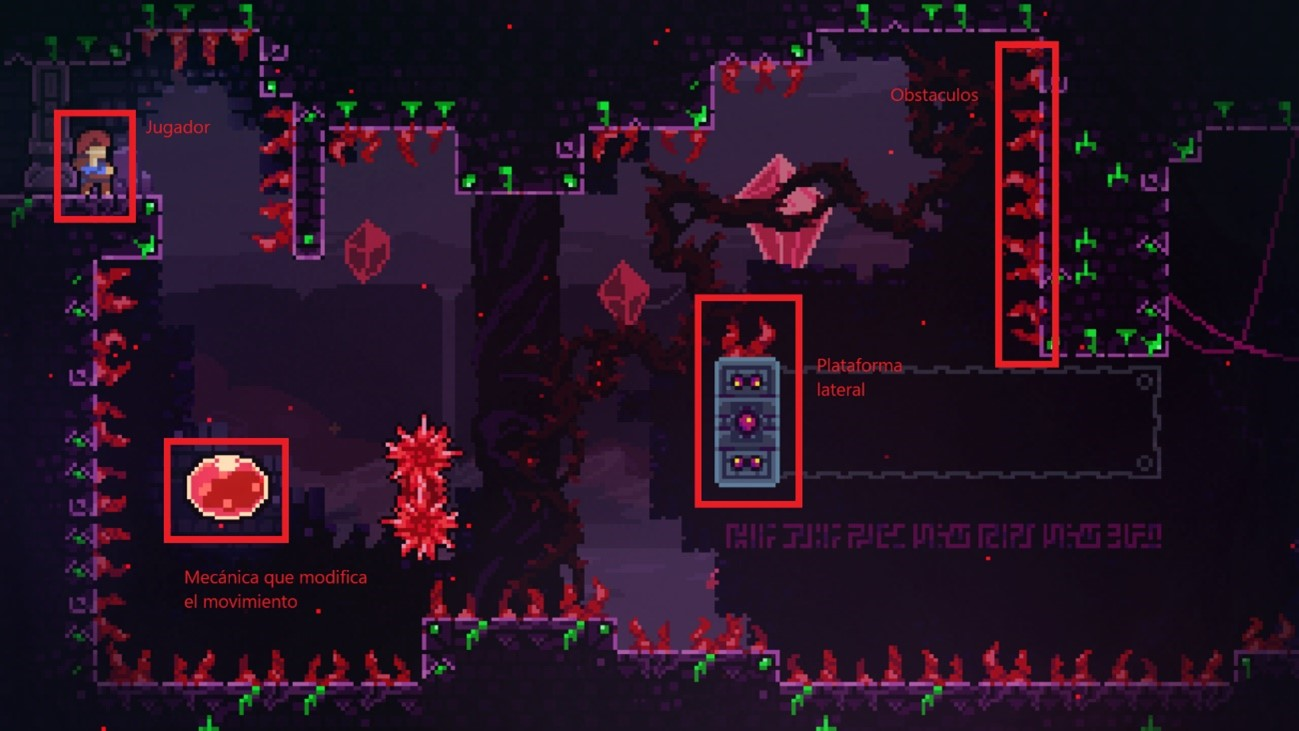
\includegraphics[scale=0.6]{Memoria/Trabajos_relacionados/Celeste}
\caption{Captura de pantalla de un nivel del videojuego Celeste.}
\end{figure}

El videojuego Super Meat Boy está muy concienciado con el movimiento del jugador. La calidad de este juego es tal, que el jugador es en todo momento consciente de donde está el avatar que controla y qué está haciendo. El juego le da mucha importancia a las físicas y como el jugador interactúa con ellas. Estas físicas no cambian, pero son un elemento muy bien establecido e intuitivo. En varios niveles el jugador tiene que hacer uso de las físicas y la inercia para superar obstáculos que en condiciones normales no sería capaz de superar.

\begin{figure}[h]
\centering
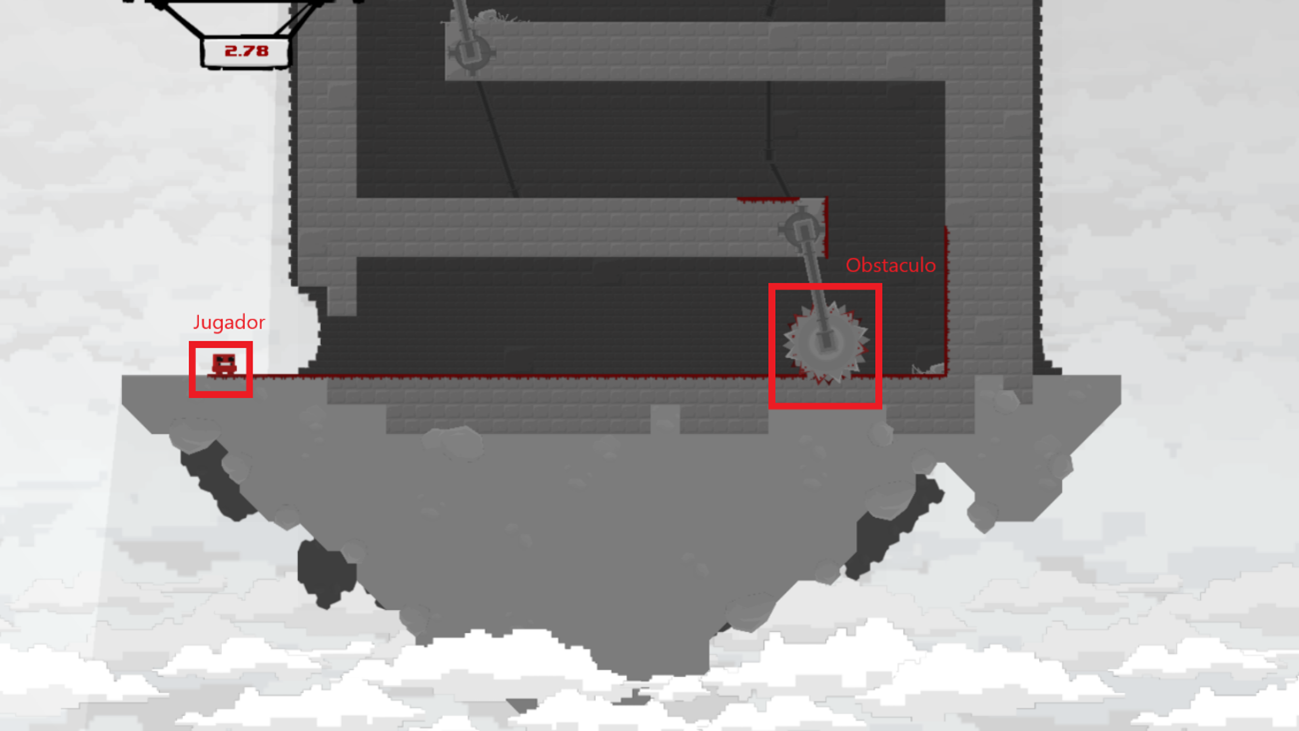
\includegraphics[scale=0.7]{Memoria/Trabajos_relacionados/Super_meat_boy}
\caption{Captura de pantalla de un nivel del videojuego Super Meat Boy.}
\end{figure}

En cuanto a la estructura de los niveles, Celeste y Super Meat Boy difieren ligeramente. En Celeste el nivel está dividido en subniveles que no tiene por qué ser independientes entre sí. El jugador escoge un capítulo y ese capítulo está dividido en una serie de niveles por los que el jugador viaja hasta alcanzar el último nivel y superar el capítulo. En la captura de pantalla anteriormente mostrada se puede observar cómo cada nivel de Celeste es cerrado, con unos límites definidos y una entrada y salida clara. El nivel generalmente se superará resolviendo un puzle que se manifiesta deduciendo un camino que requerirá el uso de distintas mecánicas para recorrerlo y llegar al siguiente nivel.

Los niveles de Super Meat Boy, como se puede observar en la captura de pantalla, no están limitados al alcance de la cámara, sino que la meta todavía no se ve. En el nivel mostrado en la captura se muestra un camino claro a seguir, pero no tiene por qué ser así.

A diferencia de Celeste, los niveles de Super Meat Boy son independientes entre sí y la salida de un nivel no es la entrada a otro, mas es cierto que se sigue una temática en la que los niveles siguen un patrón visual similar. 

Con el videojuego que se va a desarrollar se desea seguir una estructura de niveles similar a Super Meat Boy, con niveles abiertos, independientes entre sí y que no están limitados a la visión de la cámara.
Para las mecánicas se va a seguir el ejemplo de Celeste, incluyendo mecánicas visuales y variadas que generen interacción entre sí.

La temática y mecánicas de modificación de las físicas y el tiempo es la parte original que se va a implementar en el videojuego que se va a desarrollar. Mencionar aun así, que se van a utilizar mecánicas que no son enteramente originales (como el tiempo bala que se utiliza en otros géneros y en algunos otros juegos de plataformas) pero que se van a adaptar al género de plataformas 2D.

Existe un juego de plataformas 2D que se llama Braid \footnote{Página de la Wikipedia de Braid: \url{https://es.wikipedia.org/wiki/Braid}} e implementa mecánicas de viajes en el tiempo. Sin embargo, este juego tiene una temática más seria y sus mecánicas de viaje en el tiempo están más enfocadas a la resolución de un puzzle que en el disfrute inherente a usarlas con maestría. Al tener una intención tan distinta no se considera un buen referente.

\section{Evaluación de Plataformer Microgame \cite{PlatformerMicrogame}}
Para el desarrollo del videojuego se planteó partir de una plantilla de proyecto que proporcionase las bases del videojuego. Como plantilla de partida se eligió Plataformer Microgame y se realizó un estudio de la platilla para ver si era válida como punto de partida. Del estudio se obtuvo un análisis de los elementos que ofrece Plataformer Microgame.

\begin{figure}[h]
\centering
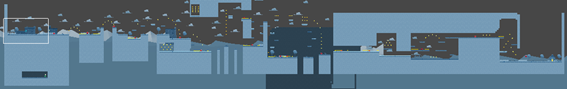
\includegraphics[scale=0.7]{Memoria/Trabajos_relacionados/Nivel_Platformer_Microgame}
\caption{Nivel de presentación de Platformer Microgame}
\end{figure}

\subsection{Grid}
Unity tiene un objeto que es el Tilemap. Este objeto permite de manera sencilla representar escenarios a partir de sprites añadidos al editor de Tilemaps. Grid es un objeto formado por una serie de Tilemaps (Foreground, Background, FarBackground y level) para formar el escenario de la escena del nivel.

\subsection{UI Canvas}
Ofrece una plantilla como punto de partida para la creación de elementos UI (User Interface).

\subsection{Enemies}
Objeto que agrupa todos los enemigos en un objeto para tenerlos centralizados y fácilmente alcanzables e identificables. En la plantilla de Platformer Microgame hay un tipo de enemigo implementado por defecto, que es el mostrado en la escena de muestra de la herramienta. Los enemigos pueden estar estáticos en un punto o seguir un patrón de movimiento.

\subsection{Tokens}
Son los típicos coleccionables de los juegos. Estos tokens tienen dos scripts que se encargan de ellos: uno para manejar las animaciones y otro para la colisión y recolección del coleccionable por parte del jugador.

\subsection{Zones}
Objeto encargado de agrupar todas las zonas de interés del nivel. Un ejemplo de estas zonas serían las zonas de victoria y de muerte del nivel (si el jugador toca la zona de victoria ganará y si toca la de muerte morirá).

\subsection{GameController}
Contiene los elementos necesarios para el funcionamiento del juego como conjunto. Principalmente contiene una clase con datos que las clases del nivel utilizaran, una clase encargada de animar los coleccionables (tokens) y una clase encargada de mostrar u ocultar el menú de pausa del juego.

\subsection{Player}
Objeto que representa el avatar que controlará el jugador.

\subsection{Simulation}
La clase Simulatión es una clase muy útil con una subclase Events. La clase Simulation tiene una cola en la que se encolarán eventos (clases que hereden de Simulation.Event). En cada frame se reproducirán todos los eventos encolados pendientes de ejecutarse.

Se explica en profundidad el funcionamiento de esta clase en el anexo C.

\subsection{Pegas}
Hay una serie de pegas importantes que se han encontrado en la plantilla de Plataformer Microgame y que han sido importantes a la hora de elegir si utilizarla o no.

\subsubsection{AnimationController}
AnimationController es la clase que implementas las físicas y la animación de los objetos (en la escena solo se aplica a los enemigos).
Esta clase se encarga de animar y controlar las físicas de los enemigos. Se viola el principio de responsabilidad única, además con dos mecánicas muy distintas como son las físicas y las animaciones. Debería separarse en dos clases distintas, una para la animación y otra para las físicas. Esto es importante porque, actualmente, en caso de querer variar las físicas o las animaciones de un enemigo tienes que reescribir todo el método ComputeVelocity() modificando tanto físicas como animaciones. El script PlayerController adolece de los mismos problemas. 
Adicionalmente delega a la animación el movimiento de todo el enemigo, lo cual obliga a las animaciones a encargarse del movimiento, tarea que no le corresponde.

\subsubsection{Health}
Health hereda de MonoBehaviour, pero no tiene necesidad de heredar de esta clase, ni heredar sus métodos y responsabilidades. La única función que sobrescribe de MonoBehaviour es Awake, función que puede ser perfectamente sustituida por un constructor. Adicionalmente, Health no tiene un método para devolver la salud a un estado inicial o por defecto, haciendo que tanto a la hora de restablecer la salud de un objeto como a la hora de restablecer la salud del Player cuando reaparece después de morir, se aplique el método Increment, método que no corresponde a esa acción.

\subsubsection{SpawnPoint}
SpawnPoint es un objeto de la escena supuestamente creado para determinar el punto de aparición del jugador, sin embargo esto solo se aplica cuando el jugador muere, de manera que inicia el juego en una posición y reaparece en otra. Esto hace muy improbable que el punto de reaparición sea el mismo que el punto en el que apareces al entrar a la escena, lo cual (en este tipo de juegos) no tiene sentido.

\subsubsection{JumpState}
La clase PlayerController maneja los estados de salto mediante una enumeración, manejándolos mediante un switch. Esto viola el principio Open/Close y centraliza todas las operaciones correspondientes a los estados en PlayerController agrandando la clase. 
En lo relativo a la acción de salto el atributo de deceleración (jumpDeceleration) del salto solo se aplica si no se mantiene el botón de salto pulsado hasta el fin de la acción de salto. Esto hace que el salto corto aplique la deceleración pero el salto largo no, de manera que la misma acción puede desenvolverse de dos formas distintas. 

\subsubsection{Rigidbody2D.Cast}
El Player utiliza el método Cast() de su Rigidbody2D para detectar los elementos que tiene a su alrededor y actuar en consecuencia. Esto provoca que todas las superficies con las que choca sean tratadas iguales, ya sean paredes o suelo, lo que desemboca en que el jugador al saltar mientras está al lado de una pared “colisione” con ella y cancele el salto a mitad de la acción. Adicionalmente puede ser un inconveniente utilizar este método a la hora de añadir mecánicas como trepar por las paredes o deslizarse por el suelo. 

\subsubsection{PatrolPath.Mover}
Los métodos establecen la forma de obtener la posición que ocupa el objeto en el momento, pero no hay límites explícitos que permitan saber por ejemplo si se ha terminado de ejecutar el movimiento o no. Esto no supone un problema debido a la implementación del código, pero, personalmente, sería preferible establecer unos límites convirtiendo la clase en algo similar a un iterador, que en cada paso calcule la siguiente posición del objeto.

\subsection{Conclusiones}
La clase Simulation es la base del funcionamiento del juego y los eventos la forma de interactuar con esta clase. Los eventos son clases heredadas de la clase abstracta Event. De esta forma se consigue una forma sencilla de crear eventos que interactúen con el entorno. Esto provoca que las demás clases solo tengan que determinar la situación y determinar cuándo lanzar los eventos. Se nota claramente en la separación en carpetas, ya que la carpeta Assets/Scripts/Gameplay está formada enteramente por eventos, mientras que la carpeta Assets/Scripts/Mechanics está formada de clases que determinan cuando lanzar eventos (entre otras responsabilidades de las que se pueden encargar algunas clases).

En líneas generales, salvo la clase Simulation, cuya implementación me parece correcta y muy útil, el resto de los elementos deberían ser reestructurados para adecuarse al modelo que se desea implementar. Sin embargo gracias a la utilidad de la clase Simulatión y todos los elementos visuales y de interfaz que ofrece por defecto la plantilla se ha tomado la decisión de desarrollar el videojuego partiendo de la plantilla Plataformer Microgame, eso sí, cambiando mucho la estructura de clases.

Algunos de los cambios que habría que realizar sobre las clases que ofrece la plantilla de Plataformer Microgame serían:

En el proyecto se delega a los propios sujetos (jugador y enemigos) la labor de simular las físicas que les afectan. Personalmente me parece más conveniente crear una clase a que se encargue de la simulación de las físicas y que los objetos jugador y enemigos sean los que le consulten como afectan las físicas. 

Health no debe heredar de MonoBehaviour. Adicionalmente Health debe añadir un método para devolver el estado de la salud a un estado inicial o por defecto. 

No hay una clase o un script que inicialice el estado del juego, sino que confía en el estado de la escena al ejecutarla, lo cual no me agrada, ya que si quieres añadir cosas al inicio de la ejecución de la escena, como por ejemplo una animación de aparición puede dificultar la labor o segregarlas en distintas clases (haciendo cada clase una serie de operaciones en el método Awake de la clase y obligando a esas clases a heredar de MonoBehaviour). Añadir una clase que haga esta labor de inicialización no pude empeorar la situación, solo mejorarla. 

Hacer una estructura de clases adecuadas a los estados del Player y los comportamientos asociados a estos, aplicando el patrón de diseño Estado. 

Cambiar el nombre de algunas clases cuyo nombre resulta confuso. Estas clases son: 
\begin{itemize}
\item
HeathIsZero a PlayerHealthIsZero. Este script solo se aplica al jugador no a todos los elementos cuya salud llega a cero. 
\item
AnimationController a EnemyAnimationController. Este script solo se aplica sobre los enemigos y no sobre cualquier objeto. 
\item
PlayerSpawn a PlayerSpawnAfterDeath. Este script solo se lanza cuando el jugador muere y ha de reaparecer en la escena y no cada vez que el Player aparece en la escena. El script podría conservar su nombre si se aplicase el evento PlayerSpawn también durante la aparición del Player.
\end{itemize}

